% Lo que debería contener este capítulo
% 
% Procesos de estampado
% Propiedades de materiales (Elasticidad / Plasticidad)
% Modelos constitutivos
% Método del elemento finito
% Teoría de contactos
% 
\chapter{Marco teórico}

\section{Procesos de formado}

El formado de metales incluye varios procesos de manufactura en los cuales se usa la deformación 
plástica para cambiar la forma de las piezas metálicas. La deformación es el resultado del uso de 
una herramienta que generalmente es un troquel para formar metales, mediante el cual se aplican 
esfuerzos que exceden la resistencia a la fluencia, induciendo una deformación plástica 
~\cite{groover2007}\\.

Normalmente, se aplica un esfuerzo de compresión para deformar plásticamente el metal, no obstante, 
algunos procesos de formado estiran, cortan o doblan el metal. Para que un metal sea adecuado 
como materia prima en un proceso de formado, este debe poseer ciertas propiedades mecánicas, 
tales como una baja resistencia a la fluencia y alta ductilidad, para facilitar la deformación 
plástica. Además, debe tenerse en cuenta el factor de la temperatura, mismo que determina 
la clasificación de trabajo en frío y caliente (referente a la temperatura de cristalización). 
También la velocidad de formación y el fenómeno de fricción entre la pieza metálica y el herramental 
son factores adicionales que afectan el desempeño del formado de metales.\\

\subsection{Tipos de formado}

Los procesos de formado se pueden clasificar en dos categoría generales, a saber: procesos de 
deformación volumétrica y procesos de trabajo de láminas metálicas.~\cite{groover2007}\\

Los \textbf{procesos de deformación volumétrica} se caracterizan por deformaciones significativas 
que derivan en grandes cambios de forma, y la relación entre el área superficial y el volumen 
de trabajo es relativamente pequeña. Algunos tipos de formado que entran dentro de esta 
clasificación son: rolado, forjado, extrusión y estirado. ~\cite{groover2007}\\

Los \textbf{procesos de trabajo de láminas metálicas} son operaciones de formado o preformado 
de láminas, tiras y rollo de metal. La razón entre el área superficial y el volumen del material 
inicial es alta, por lo que esta relación es un medio útil para distinguir la deformación 
de los procesos descritos anteriormente. Estas operaciones se ejecutan siempre en frío y 
se utiliza un herramental compuesto en la mayoría de los casos de un conjunto de formadores, 
conocidos comúnmente como punzones y matrices en el ámbito industrial. Se pueden 
distinguir de manera general tres tipos de operaciones que entran en esta clasificación: 
doblado, estirado y corte.~\cite{groover2007}\\

En este caso centraremos el interés en esta última clasificación, puesto que el proceso 
de formado del tubo se realiza utilizando una combinación de corte-doblado.

\subsection{Operaciones de doblado}

El doblado es un tipo de formado que consiste en deformar una hoja metálica, 
comúnmente conocidad como pieza de trabajo, alrededor de un eje, con un cierto 
radio de doblez, utilizando elementos formadores que ejercen una fuerza 
sobre la pieza.\\

En la figura \ref{fig:doblado_lamina} se puede ver un esquema simplificado 
de una operación de doblado, en la cual pueden observar algunos parámetros 
fundamentales de este proceso, tales como el radio (R) y ángulo de doblado 
($\alpha$), el espesor (t) y ancho (W) de la pieza, así como la ubicación 
cualitativa del eje neutro que usualmente se localiza en un rango de 1/3 
a 1/2 del espesor en hojas metálicas de acero.

\begin{center}
\includegraphics[scale=0.9]{src/ch2/doblado_lamina.png}
\captionof{figure}{Doblado de lámina}
\label{fig:doblado_lamina}
\end{center}

Las operaciones de doblado se realizan usando como herramientas diversos componentes 
que normalmente son conocidos como \textit{formadores}. Los métodos de doblado más 
comunes son el doblado en V, el doblado en U y el doblado de bordes.\\

En el doblado en V la lámina metálica se dobla entre el punzón o formador y una matriz 
en forma de V, como se muestra en la figura \ref{fig:doblado_v}. Los ángulos de doblado 
pueden incluir una variedad de rangos.

\begin{center}
\includegraphics[scale=0.4]{src/ch2/doblado_v.eps}
\captionof{figure}{Doblado en V}
\label{fig:doblado_v}
\end{center}

El doblado en U es muy similar al anterior, con la diferencia que el radio del doblado 
suele ser más amplio, como se muestra en la figura \ref{fig:doblado_u}.

\begin{center}
\includegraphics[scale=0.4]{src/ch2/doblado_u.eps}
\captionof{figure}{Doblado en U}
\label{fig:doblado_u}
\end{center}

El doblado de bordes involucra una carga voladiza sobre la lámina de metal. Se utiliza 
un \textit{pisador} que aplica una fuerza de sujeción $F_p$, para sostener la placa de 
metal en una posición adecuada para llevar a cabo el doblado, mientras el punzón 
se desliza en la parte del voladizo para forzar el doblado de la pieza sobre el borde 
de la matriz (ver figura \ref{fig:doblado_bordes}. Normalmente este tipo de doblado 
se limita a ángulos de 90° o menores.

\begin{center}
\includegraphics[scale=0.4]{src/ch2/doblado_bordes.eps}
\captionof{figure}{Doblado de bordes}
\label{fig:doblado_bordes}
\end{center}


\subsubsection{Tolerancia de doblado}

En el proceso de doblado es importante tomar en cuenta algunas características relativas a la 
pieza de trabajo. Tomando como referencia la figura \ref{fig:doblado_lamina}, una hoja metálica 
de espesor $t$ se dobla a través de un ángulo llamado ángulo de doblado $\alpha$. El  resultado 
es una pieza doblada con un ángulo incluido $\alpha'$, tal que $\alpha + \alpha' = 180°$. 
El radio de doblado $R$ se especifica normalmente en la parte interna de la pieza, en lugar de 
sobre el eje neutral, y se determina por el radio de la herramienta utilizada para ejecutar 
la operación. El doblado se hace sobre el ancho de la pieza de trabajo $w$. ~\cite{groover2007}\\

Si el radio de doblado es pequeño respecto al espesor del material el metal tiende a estirarse 
durante el doblado. Es importante poder estimar la magnitud del estirado que ocurre, de manera 
que la longitud de la pieza final pueda coincidir con la dimensión especificada. El problema 
es determinar la longitud del eje neutral antes del doblado, para tomar en cuenta el estirado 
de la sección doblada final. Esta longitud se llama \textit{tolerancia de doblado} y se puede 
estimar como sigue: ~\cite{groover2007}

\begin{equation}
A_b = 2\pi \frac{\alpha}{360} \left( R + K_{ba} t \right)
\end{equation}

Donde $A_b$ es la tolerancia de doblado en $mm$, $\alpha$ el ángulo de doblado en grados, 
$R$ el radio de doblado, $t$ el espesor del material y $K_{ba}$ es un factor para estimar 
el estirado. Los siguientes valores de diseño se recomiendan para $K_{ba}$: ~\cite{groover2007}

$$
\left\{
\begin{matrix}
K_{ba} = 0.33 & Si \,\,\, R<2t \\
K_{ba} = 0.5 & Si \,\,\, R>2t \\
\end{matrix} \right.
$$

Estos valores de $K_{ba}$ predicen que el estiramiento ocurre solamente si el radio de doblado 
es más pequeño en relación con el espesor de la lámina.

\subsubsection{Fuerza de doblado}

La fuerza requerida para llevar a cabo un proceso de doblado depende de la configuración del 
herramental, así como de las propiedades mecánicas y geométricas de la pieza de trabajo. 
Con la ecuación \ref{eq:fuerza_doblado} se puede estimar la fuerza máxima de doblado.

\begin{equation}\label{eq:fuerza_doblado}
F = \frac{K S_{t} w t^2}{D}
\end{equation}

Donde $F$ es la fuerza de doblado, $S_t$ la resistencia a la tensión del material, $w$ y $t$ el 
ancho y espesor de la pieza de trabajo, respectivamente, $D$ es la longitud de la parte abierta 
de la matriz, tal como se esquematiza en la figura \ref{fig:fuerza_doblado}. $K$ es una constante 
cuyo valor depende del tipo de doblado, normalmente 1.33 para doblado en V y 0.33 para doblado 
de bordes. ~\cite{groover2007}

\begin{center}
\includegraphics[scale=0.4]{src/ch2/fuerza_doblado.eps}
\captionof{figure}{Esquema de la fuerza de doblado}
\label{fig:fuerza_doblado}
\end{center}


\subsubsection{Recuperación elástica}

Cuando se diseña un troquel, es necesario considerar la recuperación elástica o \textit{springback} 
que ocurre después de la descarga, debido a que el material tiende a recuperar su forma 
inicial e implica que el ángulo de doblado en el herramental $\alpha_i$ no corresponda exactamente con el 
ángulo deseado $\alpha_f$. La recuperación elástica ocurre en todos los tipos de formado 
que implican un tipo de doblado.\\

\begin{center}
\includegraphics[scale=0.4]{src/ch2/springback.eps}
\captionof{figure}{Recuperación elástica de una pieza metálica sometida a doblez}
\label{fig:springback}
\end{center}

La relación dada entre los ángulos $\alpha_i$ y $\alpha_f$ se conoce como factor de \textit{springback} $k_R$, 
y depende de las características del material y la relación entre el radio de doblez y el espesor de la 
pieza de trabajo. La relación se puede expresar como sigue: ~\cite{schuler1998}

\begin{equation}\label{eq:factor_springback}
k_R = \frac{\alpha_f}{\alpha_i} = \frac{r_{i} + 0.5 s}{r_{f} + 0.5 s}
\end{equation}

Donde, usando como referencia gráfica la figura \ref{fig:springback}, $\alpha_i$ es el ángulo por el 
herramental, $\alpha_f$ el ángulo deseado en la pieza de trabajo (o después del springback), 
$s$ es el espesor de la pieza de trabajo, $r_{i}$ el radio interno en el herramental y $r_{f}$ el 
radio interno en la pieza de trabajo.\\

Luego, el ángulo necesario en el troquel o matriz viene dado por:

\begin{equation}
\alpha_i = \frac{\alpha_f}{k_R}
\end{equation}

El radio interior requerido en el troquel puede ser calculado como:

\begin{equation}
r_{i} = \frac{r_{f}}{1+\frac{r_{f} \cdot S_t}{s \cdot E}}
\end{equation}

Donde $S_t$ es la resistencia a la tensión del material y $E$ el módulo elástico correspondiente.\\

La ecuación \ref{eq:factor_springback} permite calcular la recuperación elástica a si se conoce 
previamente ambos radios internos (antes y después de la descarga). Pero es posible 
predecir la relación $r_i/r_f$ mediante la siguiente ecuación: ~\cite{kalpakjian2008}

\begin{equation}
\frac{r_i}{r_f} = 4 \left( C r_i\right)^3 - 3 \left( C r_i \right) + 1
\end{equation}

Donde $C$ es una constante dada por:

\begin{equation}
C = \frac{S_y}{Es}
\end{equation}

Siendo $S_y$ la esfuerzo de fluencia del material. Esta ecuación nos permite observar 
que la recuperación elástica aumenta cuando lo hacen la relación $r/s$ y el 
esfuerzo de fluencia $S_y$, así como al disminuir el módulo elástico.


\subsection{Herramentales (troqueles)}

Los herramentales utilizados en los procesos de formado (comúnmente llamados troqueles) son 
construidos teniendo en cuenta algunos aspectos elementales, a saber ~\cite{marin2009}:

\begin{enumerate}
\item Trabajo a realizar 
\item Características de la prensa
\item Material a troquelar
\item Número de piezas a producir
\end{enumerate}

\subsubsection{Tipos de troqueles}

A medida que aumentan los requerimientos del trabajo, la capacidad de las prensas, las exigencias 
de los materiales y la necesidad de producir más y mejor, también se conciben los diseños de 
troqueles con mayor complejidad y desarrollo. En ese sentido, los troqueles se pueden clasificar 
en simples, compuestos y progresivos.\\

\textbf{Simples}: estos troqueles permiten realizar solamente una operación por cada golpe o 
ciclo de la prensa, lo cual implica una bajo volumen de producción y productividad, y 
siendo normalmente necesario el uso de más de un herramental para terminar el producto.\\

\textbf{Compuestos}: permiten aprovechar la fuerza ejercida por la prensa realizando dos 
o más operaciones en cada golpe, agilizando el proceso y elevando en cierto punto 
la productividad.\\

\textbf{Progresivos}: son troqueles complejos y de gran desarrollo. Constan de una 
cantidad considerable de etapas, en cada uno de ellos se modifica la lámina con una secuencia 
establecida durante el diseño y acorde a los requerimientos del producto, de tal manera 
que al final se obtiene una o varias piezas terminadas. Naturalmente son altamente productivos, 
aunque su mantenimiento y operación es más compleja que en los casos anteriores.

\subsubsection{Componentes de un troquel}

Los componentes de un troquel varían dependiendo del tipo, pero típicamente hay elementos 
que se encuentran en casi todos los troqueles y que cumplen con funciones específicas 
en el proceso de formado.\\

\textbf{Base superior}. Contiene en su interior todas las placas y elementos que sostienen 
los punzones del troquel, está anclada a la prensa. Algunos elementos alojados en 
la parte superior son: placa porta-punzones, punzones, sufrideras, postes, pisadores, resortes, 
entre otros elementos adicionales.\\

\textbf{Base inferior}. Es el elemento sobre el cual van montados todos los componentes 
que hacen la parte de la matriz, y a su vez, está fuertemente sujeta en la bancada 
de la prensa durante la fase de trabajo. Algunos de los elementos contenidos en 
la base inferior son: placa  porta-matrices, guías, sufrideras, topes de avance, entre 
otros.\\

\textbf{Sufrideras}. La función básica de las placas superior e inferior de choque o sufrideras 
consiste en absorber sobre su superficie los sucesivos golpes de los elementos en el troquel. 
Estos impactos se producen cada vez que los punzones transforman la lámina con la matriz. Cuando 
el punzón impacta contra el material, la resistencia que opone este es transmitida a la 
superficie de las sufrideras sobre las que se apoyan las placas porta matriz y porta punzones. 
Estas placas están construidas en materiales ya templados y que conservan su tenacidad y cohesión, 
uno muy empleado es el acero SAE/AISI 1045.\\

\textbf{Porta punzones}. La finalidad de la placa porta punzones es la de alojar y fijar en 
su interior todos los punzones que lleve la matriz. Estos punzones pueden ser de cualquier 
tipo o tamaño pero han de tener una sola carcterística en común: deben estar firmemente 
sujetos y guiados en el interior de dicha placa impidiendo que puedan moverse o desprenderse.\\

\textbf{Porta matriz}. La placa porta matrices aloja y posiciona en su interior todos 
los elementos de pequeñas dimensiones que lleve la propia matriz, de esta manera dichos componentes 
quedarán ajustados en su interior.\\

\textbf{Placa pisadora}. Durante el movimiento descendente del troquel, la placa pisadora presiona 
la lámina dejándola inmovilizada antes de que los punzones lleguen a tocarla y mientras penetran 
el material y lo transforman. Una vez cortada la lámina, la función de la placa es mantener la 
pieza bien sujeta hasta que los punzones hayan salido de ella, de lo contrario, los punzones 
la arrastrarían hacia arriba sujeta a ellos, con el riesgo de fractura.\\

\textbf{Punzones}. Los punzones tienen por objeto realizar las máximas transformaciones en la lámina 
a fin de obtener piezas con una calidad acorde a las medidas requeridas, hay tanto tipos de estos 
como variantes del troquelado.\\

\textbf{Matrices}. Las matrices son los elementos complementarios a los punzones, tienen la forma 
negativa de estos.

\begin{center}
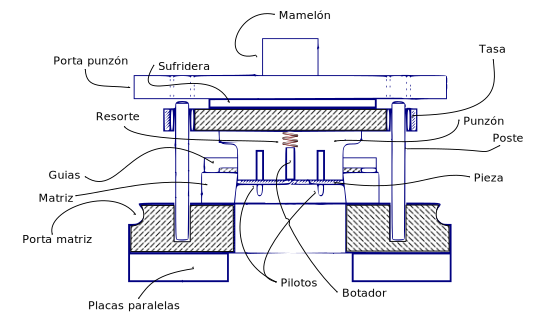
\includegraphics[scale=0.3]{src/ch2/componentes_troquel.png}
\captionof{figure}{Componentes de un troquel. \textit{Fuente:} ~\cite{wikiTroquel2008}}
\label{fig:componentes_troquel}
\end{center}


\section{Teoría de plasticidad}

La teoría de plasticidad estudia la fluencia de materiales bajo estados de esfuerzos complejos. Permite 
conocer si un material cederá bajo ciertas condiciones de esfuerzo y determinar el cambio en la forma o 
geometría en caso de que la fluencia ocurra. También permite usar datos de ensayos de tensión para predecir 
el endurecimiento por carga durante la deformación bajo complejos estados de esfuerzo. Estas relaciones 
son parte fundamental de los códigos de computadora utilizados para predecir la capacidad de una estructura 
para absorber impactos, así como en procesos de formado o estampado que involucran la deformación plástica de 
placas metálicas. ~\cite{hosford2005}

\subsection{Criterio de fluencia}

Un criterio de fluencia es una expresión matemática propuesta del estado de esfuerzo que causará 
la fluencia. La forma más general es: ~\cite{hosford2005}

\begin{equation}
f(\sigma_x,\sigma_y, \sigma_z, \tau_{yz}, \tau_{zx}, \tau_{xy} ) = C 
\end{equation}

Donde C es una constante del material. Para materiales isotrópicos esto puede ser expresado en 
términos de los esfuerzos principales como: ~\cite{hosford2005}

\begin{equation}
f(\sigma_1,\sigma_2,\sigma_3 )=C
\end{equation}

Para la mayoría de los metales dúctiles isotrópicos comúnmente se hacen las siguientes 
consideraciones: ~\cite{hosford2007}


\begin{itemize}
\item El esfuerzo de fluencia en tensión y compresión es el mismo.
\item El volumen permanece constante durante la deformación plástica
\item La magnitud del esfuerzo normal promedio, no afecta la fluencia.
\end{itemize}

\begin{equation}
\sigma_m=\frac{\sigma_1+\sigma_2+\sigma_3}{3}
\end{equation}

La consideración que la fluencia es independiente de $\sigma_m$ es razonable porque la deformación 
usualmente ocurre por deslizamiento o mecanismos de corte. Por lo tanto los criterios de fluencia 
para materiales isotrópicos tienen la forma: ~\cite{hosford2007}

\begin{equation}
f[(\sigma_2-\sigma_3 ),(\sigma_3-\sigma_1 ),(\sigma_1-\sigma_2 )] = C
\end{equation}

Esto es equivalente a considerar que la fluencia depende sólo del tamaño del círculo de Mohr, 
y no de su posición, la figura \ref{fig:circulos_mohr} muestra esto. Si el estado de esfuerzos 
$\sigma_1$, $\sigma_2$, $\sigma_3$, causará la fluencia, otro estado de efuerzos 
$\sigma_1' = \sigma_1 - \sigma_m $, $\sigma_2' = \sigma_2 - \sigma_m $, $\sigma_3' = \sigma_3 - \sigma_m $, 
que difiere sólo por $\sigma_m$, también causará la fluencia. Estos esfuerzos $\sigma_1'$, $\sigma_2'$, 
$\sigma_3'$ se conocen como esfuerzos desviatorios. ~\cite{hosford2007}

\begin{center}
\includegraphics[scale=0.75]{src/ch2/circulos_mohr.png}
\captionof{figure}{Círculos de Mohr para dos estados de esfuerzos que difieren por un esfuerzo hidrostático, $\sigma_m$ y que son equivalentes en términos de la fluencia}
\label{fig:circulos_mohr}
\end{center}



% =========================================== Criterio de tresca =============================================
\subsection{Criterio de Tresca}

El criterio más simple es uno de los primero propuestos por Tresca. Afirma que la cedencia 
ocurrirá cuando el máximo esfuerzo cortante alcance un valor crítico. El máximo esfuerzo 
cortante viene dado por:

\begin{equation}
\tau_{max} = \frac{\sigma_{max}-\sigma_{min}}{2}
\end{equation}

entonces, el criterio de Tresca puede expresarse como:

\begin{equation}
\sigma_{max} - \sigma_{min} = C
\end{equation}

Si se mantiene la convención de que $ \sigma_1 \me \sigma_2 \me \sigma_3 $, puede reescribirse lo anterior como:

\begin{equation}\label{eq:ec1}
\sigma_1 - \sigma_3 = C
\end{equation}

La constante C puede ser encontrada mediante un ensayo de tensión uniaxial. En un ensayo de tensión, 
$\sigma_2 = \sigma_3 = 0$ y la cedencia $\sigma_1 = Y$, donde $Y$ es el esfuerzo de fluencia. Sustituyendo 
en $C=Y$ en la ecuación \ref{eq:ec1}. Por lo tanto el criterio de Tresca puede ser expresado como:

\begin{equation}\label{eq:ec2}
\sigma_1 - \sigma_3 = Y
\end{equation}

Para cortante puro, $ \sigma_1 = -\sigma_3 = k$, donde $k$ es esfuerzo de fluencia por cortante. Sustituyendo 
$ k = Y/2 $ en la ecuación \ref{eq:ec2}, entonces:

\begin{equation}
\sigma_1 - \sigma_3 = 2k = C
\end{equation}

\subsection{Criterio de Von Mises}

El efecto del esfuerzo principal medio puede ser incluido asumiendo que la fluencia depende de la raíz cuadrada 
del promedio de los diámetros de los tres círculos de Mohr. Este es el criterio de Von Mises, el cual puede ser 
expresado como:

\begin{equation} \label{eq:ec3}
\left\{ [(\sigma_2-\sigma_3)^2 + (\sigma_3-\sigma_1 )^2 + (\sigma_1-\sigma_2 )^2]/3 \right\}^{1/2} = C
\end{equation}

Como cada término está elevado al cuadrado, la convención $\sigma_1 \me \sigma_2 \me \sigma_3$ no es necesaria. 
La constante del material, $C$, puede ser evaluada mediante un ensayo de tensión uniaxial. En la fluencia, 
$\sigma_1 = Y$ y $\sigma_2 = \sigma_3 = 0$. Sustituyendo, $[0^2 + (-Y)^2 + Y^2]/3 = C^2$, o 
$C = (2/3)^{1/3} Y $, entonces, la ecuación usualmente se escribe como:

\begin{equation}\label{eq:ec4}
(\sigma_2-\sigma_3)^2 + (\sigma_3-\sigma_1 )^2 + (\sigma_1-\sigma_2 )^2 = 2Y^2
\end{equation}

Para cortante puro, $\sigma_1 = -\sigma_3 = k$ y $\sigma_2=0$. Sustituyendo en la ecuación \ref{eq:ec4}, 
$ (-k)^2 + [ (-k)-k ]^2 + k^2 = 2Y^2 $, entonces:

\begin{equation}\label{eq:ec5}
k = Y/\sqrt{3}
\end{equation}

La ecuación \ref{eq:ec5} puede ser simplificada si uno de los esfuerzos principales es cero (condición de esfuerzo plano). 
Sustituyendo $\sigma_3 = 0$, $\sigma_1^2 + \sigma_2^2 - \sigma_1 \sigma_2 = Y^2$, el cual es una elipse. Con la 
consiguiente sustitución de $\alpha = \sigma_2/\sigma_1$,

\begin{equation}
\sigma_1 = Y/(1-\alpha+\alpha^2)^{1/2}
\end{equation}


\section{El método de los elementos finitos}

\subsection{Generalidades del método}

En el método de elementos finitos se considera un cuerpo continuo o sólido, como un ensamble de pequeñas 
subdivisiones llamadas elementos finitos. Estos elementos están interconectados a través de nodos comunes. 
Debido a que la variación real de las variables de campo (desplazamientos, esfuerzos, temperaturas, etc.) 
se desconoce en el continuo, se asume que la variación de estas en el modelo de elemento finito puede ser 
aproximada por una simple función. Estas funciones de aproximación, también llamadas modelos de interpolación, 
son definidas en términos de los valores nodales de las variables de campo.\\

En general, el método de los elementos finitos, consiste en formular un sistema de ecuaciones 
(ecuaciones de equilibrio) para el sistema continuo que ha sido discretizado, donde las incógnitas 
suelen ser los valores nodales de las variables de campo. Luego, se resuelve este sistema de ecuaciones, 
con las consideraciones correspondientes a las condiciones de frontera o valores iniciales que simplifiquen 
el modelo original. La siguiente ecuación muestra, en notación matricial, el sistema de ecuaciones resuelto 
en una formulación de elemento finito.

\begin{equation}
K\,\bm{u} = \bm{P}
\end{equation}

Donde $K$ es la matriz global de rigidez, $\bm{u}$ es el vector de desplazamientos nodales y $\bm{P}$ el 
vector de fuerzas nodales en el sistema.\\

Para problemas lineales, el vector $\bm{u}$ puede ser resuelto de manera sencilla, mediante 
procedimientos básicos del álgebra lineal. Sin embargo, para problemas no lineales, la solución 
tiene que ser obtenida mediante una secuencia de pasos, en el cual cada uno de estos implica la 
modificación de la matriz de rigidez $K$ y/o el vector global de carga $\bm{P}$.\\

En problemas de análisis dinámico, desplazamientos, velocidades, deformaciones, esfuerzos y cargas 
son dependientes del tiempo. Por ello deben incluirse algunos otros términos, por lo que la ecuación 
a resolver viene dada por la expresión siguiente:

\begin{equation}
M\ddot{\bm{u}} + C\dot{\bm{u}} ̇+ K\bm{u} = \bf{P}
\end{equation}

Donde $C\,\dot{u}$ representa las fuerzas viscosas, mismas que deben incluirse cuando el 
sistema esté amortiguado artificialmente.



\subsection{Solución implícita vs explícita}

Existen, de manera general, dos tipos de métodos para resolver ecuaciones diferenciales  
en problemas dependientes del tiempo: integración implícita e integración explícita. El 
método implícito de integración en el tiempo puede ser expresado como: ~\cite{nielsen1997}

\begin{equation}
u_{n+1}=f(\dot{u}_{n+1},\ddot{u}_{n+1},u_n,\dot{u}_n,…)
\end{equation}

y el método explícito como:

\begin{equation}
u_{n+1}=f(u_n,\dot{u}_n,\ddot{u}_n,u_{n-1},\dot{u}_{n-1},…)
\end{equation}

El método implícito requiere conocer las derivadas temporales en el paso n+1, las cuales son desconocidas, 
mientras el método explícito está basado en los valores conocidos en el paso n. Si el problema es no 
lineal, el método implícito necesita un procedimiento iterativo para determinar los nuevos desplazamientos. 
Con el método explícito los nuevos desplazamientos se determinan directamente de los valores conocidos 
en pasos previos, evitando el uso de iteraciones adicionales.~\cite{nielsen1997}\\

La simulación de estampados se caracteriza por las diversas no linealidades presentes, debidas al 
material, y a los contactos entre los diversos cuerpos analizados. Sin embargo, usando la integración 
explícita estas no linealidades pueden ser tratadas sin mayores problemas. Por ello, en la mayoría de 
las simulaciones de estampados suelen ser conveniente el uso de algoritmos de integración explícita.


\subsection{Contactos}
